\documentclass[11pt]{report}
\usepackage{fullpage}
%\usepackage{sourcesanspro, sourcecodepro}
\usepackage{minted}
\usepackage{graphicx}
\usepackage{awesomebox}
\usepackage{hyperref}

\hypersetup{
    colorlinks=true,
    linkcolor=blue,
    citecolor=blue,
    filecolor=blue,
    urlcolor=blue,
    pdfborder={0 0 0}
}

\graphicspath{{./images/}}

\title{APSC 258: Lab 1 Manual}
\author{Andre Cox}

\begin{document}
    \maketitle
    \tableofcontents

    \chapter{Introduction}

    \section{Authors Note}
    The lab manuals written in a way that not only guides you through the lab, but also provides you with interesting examples of how we can apply the concepts learnt to real world problems that you may encounter in your engineering career. For the best learning experience, it's recommended to read over the lab manuals before starting the lab.
    As well there may not always be one correct answer to a problem and there may be many different ways to solve a problem. Lot's of parts of the lab require some trial and error so don't be discouraged if you don't succeed at your first attempt.


    \section{Background}
    Engineers are often designing complex systems that require a lot of time and effort to build such as self driving cars, and machines that can process and understand data in a comprehensive way.
    Luckily for us, we have the power of machine learning to help us solve these problems. Currently machine learning has become easily accessible to engineers and researchers so in the following labs we will set out to create our own machine learning models to create a simple self driving car.
    Although our models will be relatively simple, the techniques you will learn can be applied to every engineering discipline to solve problems that appear very complex.

    \section{Introducing the Self Driving Car Project}
    Over the course of the semester we will be creating a rudimentary self driving car. As it is impractical to use a car to drive around in the real world, we will use a small Remote Controlled Car. This car will have a camera that can see the "road" which we will be made of painters tape. At the end of the semester we will have a competition to see how capable each teams car is.

    \chapter{Start of the Lab}

    \section{Introducing the Pi Car}
    When you come to your first lab you will be given the PiCarV a remote controlled car with a computer built right in! 

    % show image
    \begin{figure}[h]
        \centering
        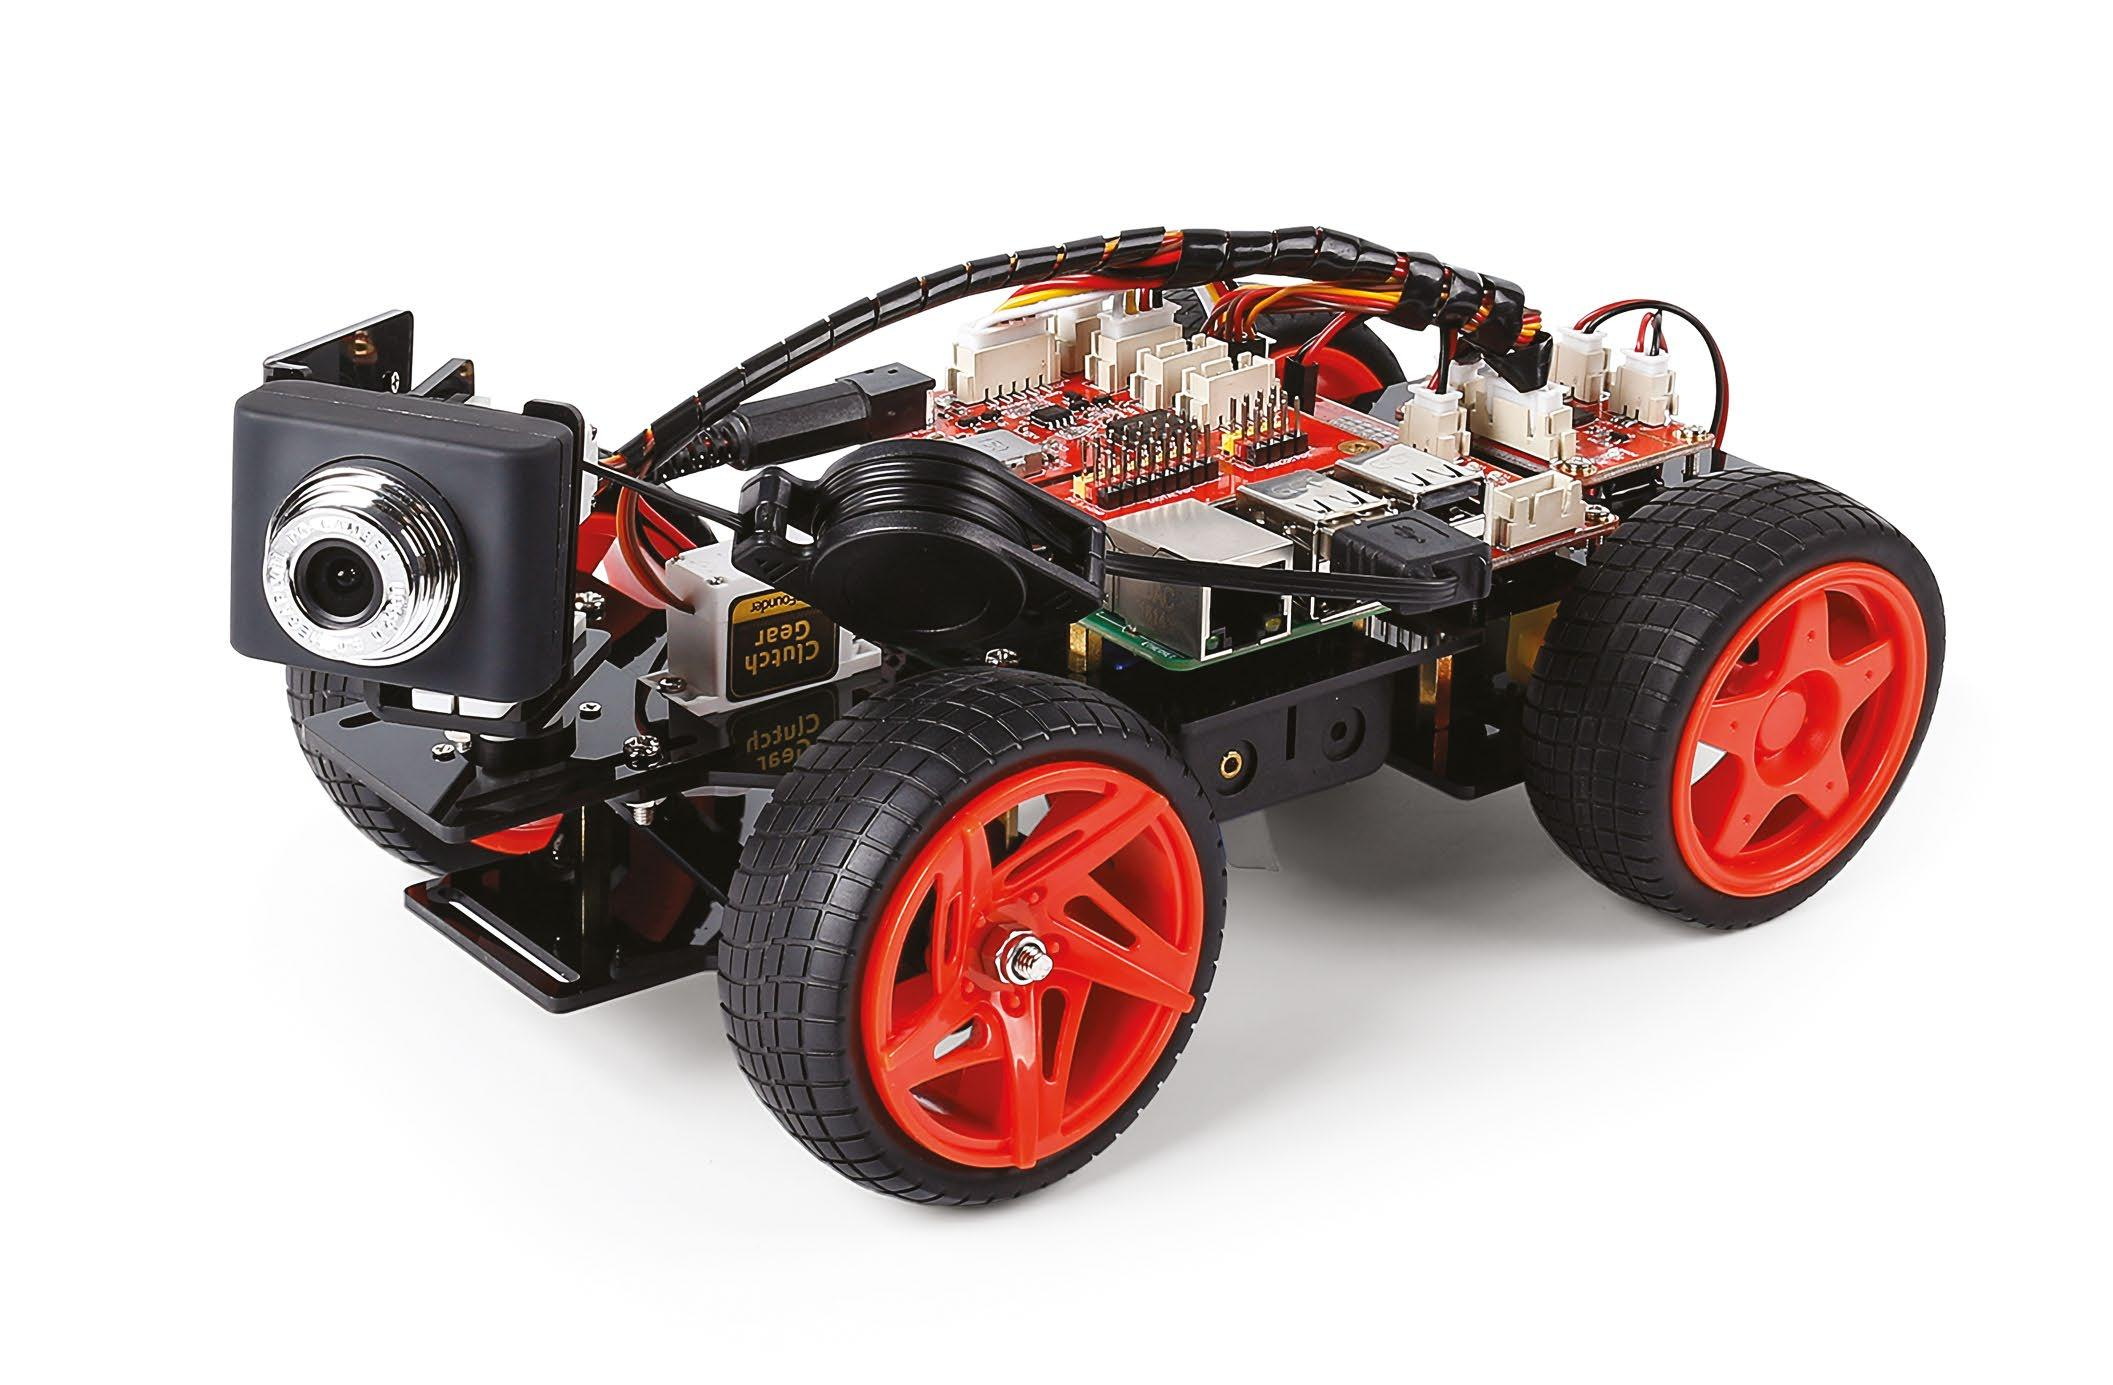
\includegraphics[width=0.8\textwidth]{picarv.jpg}
        \caption{The Assembled PiCarV}
        \label{fig:The Assembled PiCarV}
    \end{figure}

    The first thing to do is to check if you have received all the components. The PiCarV should already be Assembled and ready to go so make sure you have these components.

    \begin{itemize}
        \item 18650 Lithium-Ion Battery x2 (They should be wrapped in plastic, do not remove this!)
        \item 18650 Charger x1
        \item 18650 Charger Cable x1
    \end{itemize}

    As well you should look out to make sure nothing is obviously broken and no cables are unplugged.

\begin {figure}[h]
    \centering
    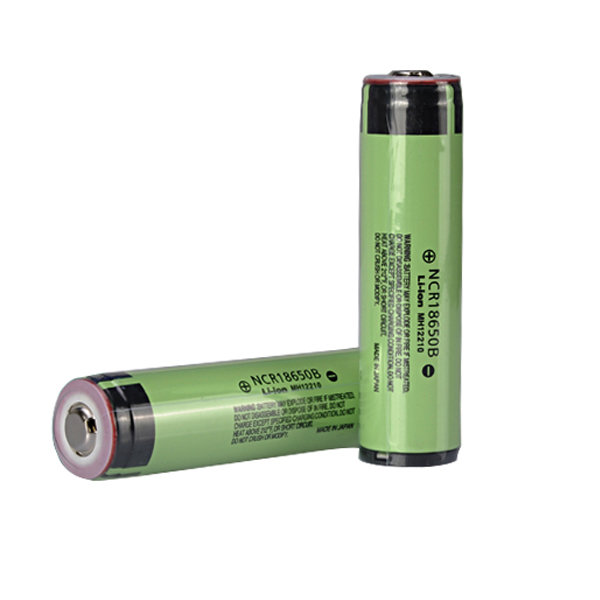
\includegraphics[width=0.5\textwidth]{battery.jpg}
    \caption{18650 Battery}
    \label{fig: 18650 Battery}
\end{figure}
    
\notebox{
    \textbf{18650 Facts:}
    The 18650 Battery Cell is one of the most common battery cells in the world. They are used in almost every electric car and bike. They can be connected together in series and parallel to create any battery pack an engineer may need. From a small 2 cell battery pack like in our PiCarV to a full size electric car with over 8000 cells.
}

\section{Testing the PiCarV}
To test the PiCarV you will first need to charge the batteries by placing them in the charger. Your charger has 2 buttons on the front, you do not need to touch these.

\cautionbox{
    \textbf{Warning Fire Hazzard:}
    While 18650 batteries are generally very safe, under the wrong circumstances they can cause a fire hazard. To alleviate this you should always be present when charging the batteries and make sure you store the batteries away from flammable materials. As well the cells should be kept away from the heat source. For instance do not leave the batteries in a hot car.
}

Once the charger has finished the batteries can be placed into the PiCarV. Next switch on the PiCarV. You should see the lights on the side of the PiCarV start to blink. You can check if everything is working by opening your WiFi settings on your phone or laptop and checking if a hotspot has been created. It should be called PiCarV followed by a string of letters and numbers. Write this down as it can be hard to know what hotspot to connect to when lots of PiCars are running at the same time.

\section{Connecting the controller to the PiCarV}
We provide a simple controller app that you can use to check that your PiCarV is working. You can download the app from the following link. 
% include hyperlink
\href{https://github.com/PiCarV/Controller/releases}{PiCar Controller} Make sure you get the correct version for your operating system. EXE for windows and DMG for mac.


Once you have installed the controller you can connect your computer to the PiCar hotspot the password is "raspberry". Next you can open the controller app and enter in the IP address of the PiCarV in the top right corner. The IP address is "192.168.0.10". Once this is entered the text that says "connected: false" should change to "connected: true" and you should see a live stream from the camera. Try to have a go controlling the PiCarV with the wasd or arrow keys. 

% show image
\begin{figure}[h]
    \centering
    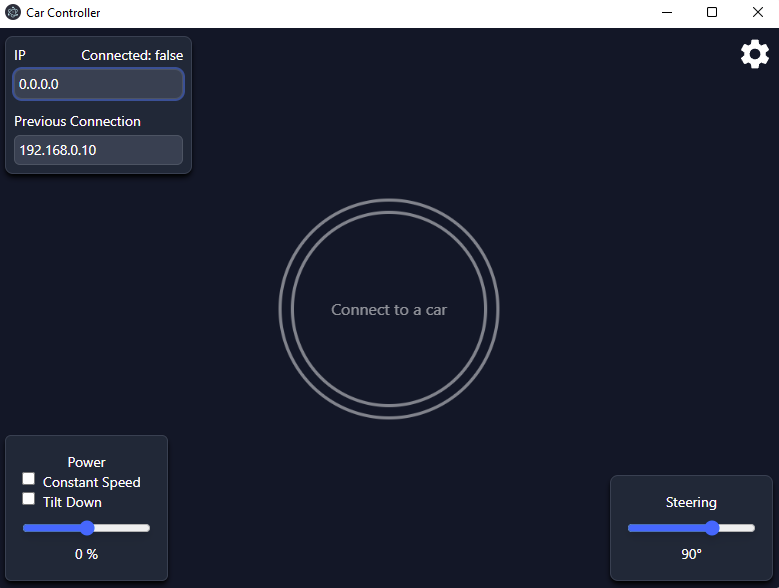
\includegraphics[width=0.8\textwidth]{controller.png}
    \caption{Controller}
    \label{fig:Controller}
\end{figure}

\chapter{Finishing Up}
Now we can control the PiCar through a simple application. The PiCar is ready for your next lab where you will learn how to send your own commands to run the PiCar using Python.

\end{document}




